% Autor: Simon May
% Datum: 2017-10-05
% Diese Datei bietet ein minimalistisches Grundgerüst für ein LaTeX-Dokument,
% z.B. für die Bearbeitung der Aufgaben.
\documentclass[
	% Papierformat
	a4paper,
	% Schriftgröße (beliebige Größen mit „fontsize=Xpt“)
	12pt,
	% Schreibt die Papiergröße korrekt ins Ausgabedokument
	pagesize,
	% Sprache für z.B. Babel
	ngerman
]{scrartcl}

% Achtung: Die Reihenfolge der Pakete kann (leider) wichtig sein!
% Insbesondere sollten (so wie hier) babel, fontenc und inputenc (in dieser
% Reihenfolge) als Erstes und hyperref und cleveref (Reihenfolge auch hier
% beachten) als Letztes geladen werden!

% Silbentrennung etc.; Sprache wird durch Option bei \documentclass festgelegt
\usepackage{babel}
% Verwendung der Zeichentabelle T1 (Sonderzeichen etc.)
\usepackage[T1]{fontenc}
% Legt die Zeichenkodierung der Eingabedatei fest, z.B. UTF-8
\usepackage[utf8]{inputenc}
% Schriftart
\usepackage{lmodern}
% Zusätzliche Sonderzeichen
\usepackage{textcomp}

% Mathepaket (intlimits: Grenzen über/unter Integralzeichen)
\usepackage[intlimits]{amsmath}
% Ermöglicht die Nutzung von \SI{Zahl}{Einheit} u.a.
\usepackage{siunitx}
% Zum flexiblen Einbinden von Grafiken (\includegraphics)
\usepackage{graphicx}
% Abbildungen im Fließtext
\usepackage{wrapfig}
% Abbildungen nebeneinander (subfigure, subtable)
\usepackage{subcaption}
% Funktionen für Anführungszeichen
\usepackage{csquotes}
% Zitieren, Bibliographie
\usepackage{biblatex}

% Verlinkt Textstellen im PDF-Dokument
\usepackage[unicode]{hyperref}
% "Schlaue" Referenzen (nach hyperref laden!)
\usepackage{cleveref}

% siunitx: Deutsche Ausgabe, Messfehler getrennt mit ± ausgeben
\sisetup{
	locale=DE,
	separate-uncertainty
}

\begin{document}
\begin{titlepage}
	\centering
	{\scshape\LARGE Versuchsbericht zu \par}
	\vspace{1cm}
	{\scshape\huge E4\par}
	\vspace{2.5cm}
	{\LARGE Gruppe 2 Mo\par}
	\vspace{0.5cm}
	{\large Nils Kulawiak (E-Mail: n\_kula01@wwu.de) \par}
	{\large Oliver Brune (E-Mail: o\_brun02@wwu.de) \par}
	\vfill
	durchgeführt am 15.1.2017\par
	
	\vfill

	{\large \today\par}
\end{titlepage}


\tableofcontents
	
	
\newpage
\section{Einleitung}
Ziel dieses Versuches ist es die Phasenumwandlung einer Kupfer-Gold Mischung für verschiedene Temperaturen zu untersuchen, wobei bekannt ist, dass es sich um ein fcc-Gitter handelt. Im ersten Teil des Versuchs wird das erreicht, indem diese Mischung unter sich verändernden Winkel mit Röntgenstrahlung bestrahlt wird und die Intensität dazu gemessen wird. Wenn es zu einer konstruktiven Interferenz kommt, kann mithilfe der Bragg-Gleichung auf den Abstand der Ebenen voneinander geschlossen werden:
\begin{equation}
2d sin(\theta) = n \lambda
\label{bragg}
\end{equation}

Wenn bekannt ist um was für eine Ebene es sich handelt, kann daraus wiederum der Gitterabstand eines kubischen Gitters berechnet werden.

\begin{equation}
d = \frac{a}{\sqrt{h^{2}+k^{2}+l^{2}}}
\end{equation}

Damit lässt sich daraufhin zeigen, wie sich der Gitterabstand mit der Temperatur verändert, wobei ein linearer Anstieg erwartet wird.

Außerdem soll versucht werden die sogenannte Fernordnung zu bestimmen, welche aussagt wie geordnet ein Kristallgitter ist. Ein fcc-Gitter lässt sich in vier verschiedene sc-Gitter aufteilen. Bei einer vollständigen Ordnung befinden sich alle Goldatome auf dem sc-Gitter mit der Basis (0,0,0), während sich die Kupferatome auf den anderen drei sc-Gitter befinden.
Bei einer vollständigen Unordnung ist es rein zufällig, wie die Gold und Kupferatome verteilt sind.

Um die Fernordnung zu bestimmen, muss zuerst die Intensität theoretisch bestimmt werden. 
Dies passiert bis auf eine Konstante genau mit
\begin{equation}
I_{hkl} \propto |F_{hkl}|^{2} \cdot p \cdot L_{p} \cdot D_{T}.
\end{equation}

\begin{itemize}


\item Der Flächenhäufigkeitsfaktor p beschreibt dabei wie häufig eine Ebene in der Gitterstruktur vorkommt.

\item Der Lorentz-Polarisationsfaktor $L_{p}$ korrigiert verschiedene Effekte der Röntgenbeugung und beträgt $L_{p} =\frac{1 + cos^{2}(2 \theta)}{sin^{2}(\theta) cos(\theta)}$. 

\item Der Debye-Waller-Faktor beschreibt den Einfluss der Wärmebewegung auf die Intensität und beträgt $D_{T} = \text{exp}(-2B \cdot \frac{sin^{2}(\theta)}{\lambda^{2}})$, wobei B ein experimentell bestimmter Wert ist.

\item Der Strukturfaktor $F_{hkl}$ beschreibt das Streuvermögen einer Elementarzelle.
\end{itemize}

Um den Streufaktor zu berechnen wird über alle Basisatome summiert.
\begin{equation}
F_{hkl} \propto \sum_{i=1}^{n} f_{i} e^{2 \pi i(hx_{i} + ky_{i} + lz_{i})}
\end{equation}

Da sich die Basisatome bei $(0,0,0) ; (\frac{a}{2},\frac{a}{2},0) ; (\frac{a}{2},0,\frac{a}{2})$ und $(0, \frac{a}{2}, \frac{a}{2})$ befinden, ergibt sich der Streufaktor bei vollständiger Ordnung zu 
\begin{equation}
F_{hkl} = f_{Au} + f_{Cu} (e^{2 \pi i(h+l)} + e^{2 \pi i(k+l)} + e^{2 \pi i(h+k)}).
\end{equation}

Somit ergibt sich für jede Ebene ein Peak, allerdings sind die Peaks mit nur geraden oder ungeraden h,k und l deutlich größer, da der Strukturfaktor dort $f_{Au} + 3f_{Cu}$ ergibt und sonst $f_{Au} - f_{Cu}$.

Anders verhält es sich bei der vollständigen Unordnung. Dort ergibt sich der Strukturfaktor zu 
\begin{equation}
F_{hkl} = (\frac{1}{4} f_{Au} + \frac{3}{4}f_{Cu}) (1 + e^{2 \pi i(h+l)} + e^{2 \pi i(k+l)} + e^{2 \pi i(h+k)}).
\end{equation}

Somit bleibt der Strukturfaktor gleich für alle h,k und l gerade oder ungerade, allerdings ergibt sich der Strukturfaktor für alle anderen Ebenen zu 0. 
Die Röntgenreflexe, die immer unabhängig von der Fernordnung erscheinen, nennt man Fundamentalreflex, während die sich ändernden Überstrukturreflex genannt werden.

Unter der Annahme, dass der Strukturfaktor linear mit der Fernordnung $\mu$ skaliert ergibt er sich zu
\begin{equation}
F_{hkl} = \left \{ \begin{array}{ll}
f_{Au} + 3f_{Cu} \text{  für nur gerade oder ungerade h,k,l} \\
\mu (f_{Au} - f_{Cu}) \text{  sonst} \\
\end{array} \right .
\end{equation}

Daraus lässt sich dann die Fernordnung berechnen  mit 
\begin{equation}
\mu^{2} = \frac{I^{Ü}(\mu)}{I^{Ü}(1)} = \frac{I^{Ü}_{exp}(\mu)\cdot I^{F}_{theo}}{I^{F}_{exp} \cdot I^{Ü}_{theo}(1)}.
\end{equation}  

Außerdem sollen noch die Kernaussagen von Debye überprüft werden. Diese heißen:
1. Die Schärfe der Interferenzmaxima wird durch die Wärmebewegung nicht beeinflusst.

2. Durch die Wärmebewegung ändert sich die räumliche Intensitätsverteilung.

3. Aufgrund der Wärmebewegung nimmt die Interferenzintensität
\begin{itemize}
\item mit zunehmender Temperatur 
\item mit zunehmendem Winkelabstand zwischen Einfalls- und Beobachtungsrichtung 
\item mit abnehmender Wellenlänge
\end{itemize}
exponentiell ab.
\section{Erhöhung der Temperatur}
\subsection{Ergebnis}
Um herauszuf

\begin{figure}[h]
	\centering
	\includegraphics[scale=0.35]{25.PNG}
	\caption{Intensitätsverteilung bei Raumtemperatur}
	\label{ski}
\end{figure}

\section{Kalorimetrie}
\subsection{Methoden und Durchführung}
Zur Analyse des Phasenübergangs in der CuAu-Legierung wird eine kalorimetrische Untersuchung durchgeführt. Hierfür wird ein dynamisches Wärmestromdifferenzkalorimeter, zu sehen in \cref{kalori}, verwendet. Mit diesem werden Temperaturdifferenzen zwischen einer Probe und einer Referenz gemessen, die sich beide in einem Aluminiumtiegel befinden. Die Differenz ist in diesem Versuch einfach ein leerer Tiegel (Luftreferenz). Beide befinden sich dabei in einer Kammer, in der sie symmetrisch auf einer Scheibe positioniert werden ("disk-type"). Wenn die Kammer nun aufgeheizt wird, kann über die Scheibe die Temperaturdifferenz zwischen den beiden Proben ermittelt werden.

\begin{figure}[h]
	\centering
	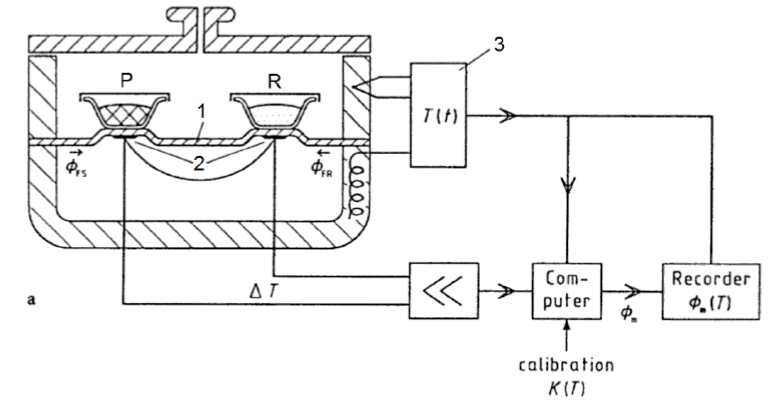
\includegraphics[scale=0.7]{Kalorimeter.png}
	\caption{Aufbau eines "disk-type" Wärmestrom-DSC. P: Probe, R: Referenz, 1: Scheibe,
		2: Thermoelemente, 3: Temperaturregelung.}
	\label{kalori}
\end{figure}

In diesem Versuch wird die Methode verwendet um den Phasenübergang zwischen Ordnung und Unordnung in der CuAu-Legierung zu untersuchen. Hierfür wird die Kammer zuerst auf eine Temperatur von $\SI{500}{\degreeCelsius}$ gebracht. Diese liegt deutlich über der Phasenübergangstemperatur, deswegen ist der Kristall in diesem Zustand ungeordnet. Anschließend wird die Kammer wieder abgekühlt, zuerst auf $\SI{410}{\degreeCelsius}$ mit einer Rate von $\SI{60}{\degreeCelsius/\minute}$, anschließend sehr langsam mit einer Rate von $\SI{5}{\degreeCelsius/\minute}$ auf $\SI{385}{\degreeCelsius}$. Diese Temperatur liegt knapp unter der Phasenübergangstemperatur von $\SI{390}{\degreeCelsius}$, daher ist nun der Phasenübergang der Legierung zu erwarten. Um diesen zu beobachten, wird die Temperatur nun für $\SI{30}{\minute}$ konstant gehalten. Der Phasenübergang von Unordnung zu Ordnung ist ein exothermer Vorgang, das heißt die Probe gibt dabei Wärme ab. Dieser Wärmefluss kann über die Temperaturdifferenz bestimmt werden. Da der Wärmefluss ein Maß für die Änderung des umgewandelten Volumens im isothermen Phasenübergang ist, kann mit diesem untersucht werden, inwiefern die Versuchsergebnisse mit der Johnson-Mehl-Avrami-Kolmogorow-Gleichung (\cref{eq:jmak}) übereinstimmen. Insbesondere soll betrachtet werden, ob die Wahl des Avrami-Exponenten auf $n=4$ mit den Messwerten übereinstimmt.
\begin{equation}
	\frac{\mathrm{d}X(t)}{\mathrm{d}t} = H \cdot K \cdot n \cdot \exp(-K\cdot (t-t_0)^n)\cdot (t-t_0)^{n-1}
	\label{eq:jmak}
\end{equation}

\subsection{Auswertung}
In \cref{3} wurde der im Kalorimeter gemessene Wärmestrom gegen die Zeit aufgetragen. Zuerst steigt der Wärmestrom sehr stark, das liegt daran, dass sich das System erst in der Isotherme einpendeln muss, da die Kammer vorher gekühlt wurde. Dieser Vorgang dauert etwa $105$ Sekunden, an dieser Stelle ist ein lokales Maximum erreicht. Anschließend sinkt der Wärmefluss wieder, erreicht nach ca. $300$ Sekunden ein lokales Minimum und steigt dann bis etwa $450$ Sekunden nach Beginn der Isotherme auf den Wert des vorherigen lokalen Maximums. Den Rest der Zeit steigt der Wärmefluss nur noch leicht an.

\begin{figure}[hb]
	\centering
	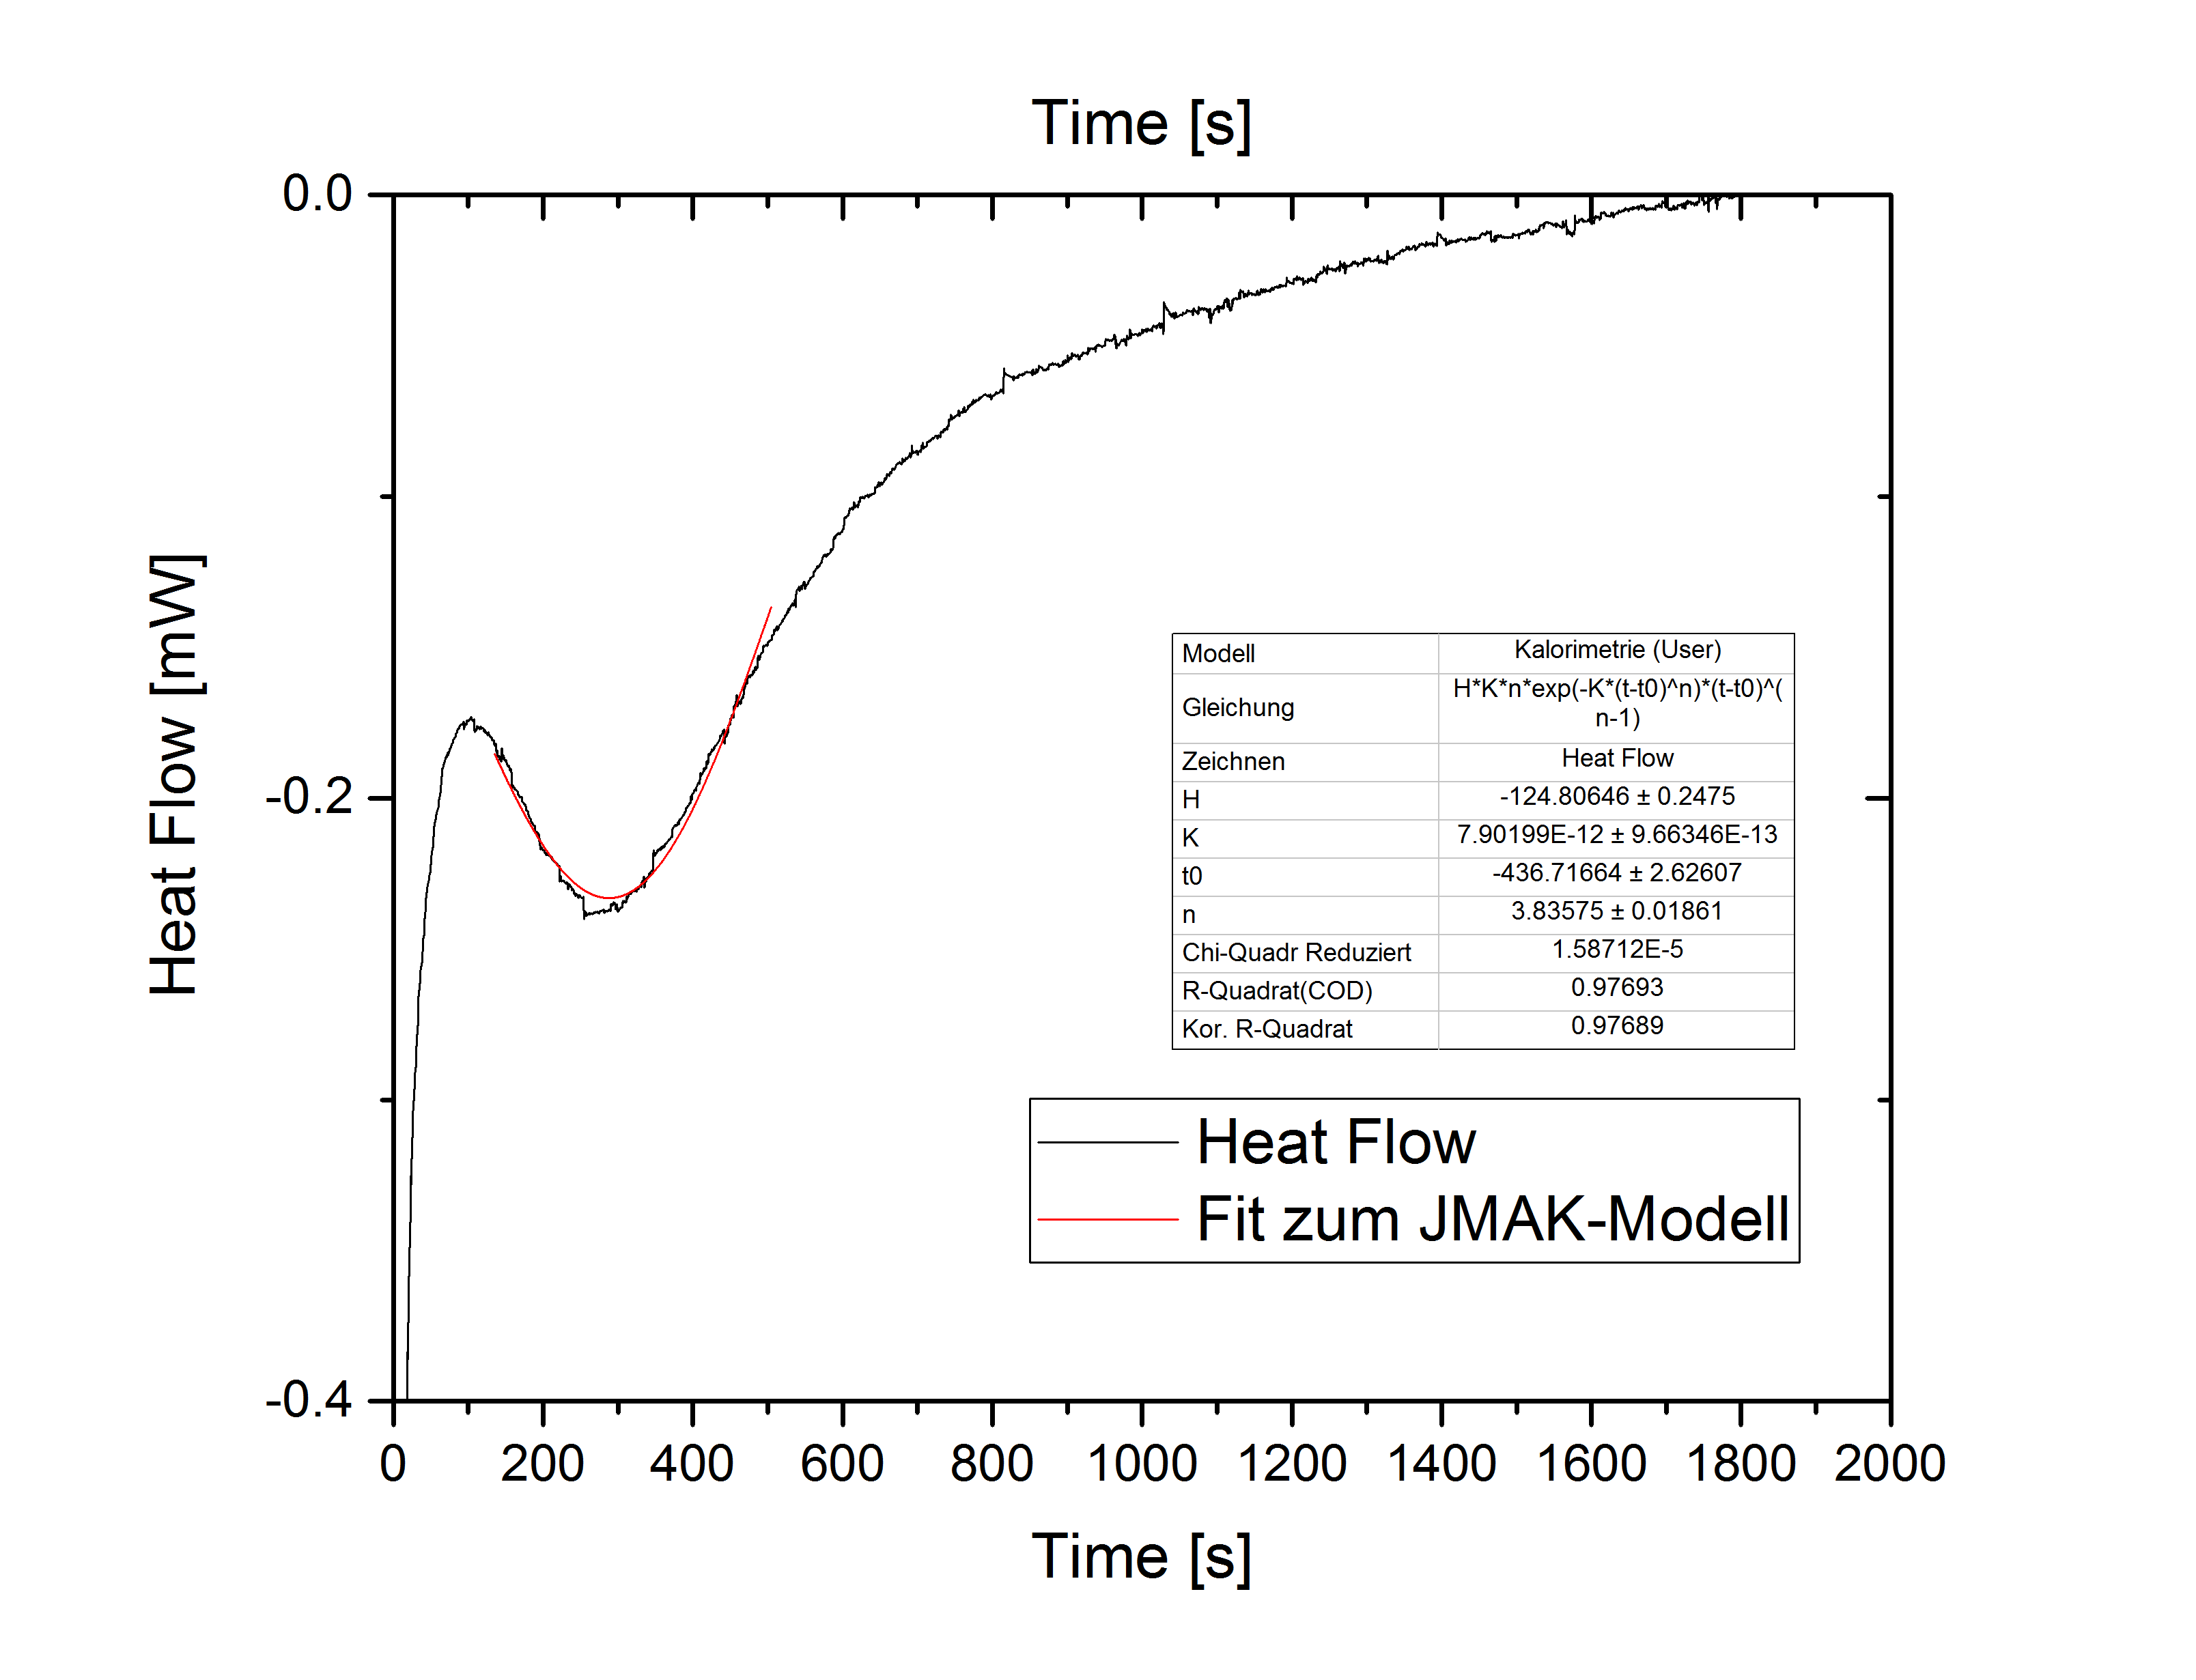
\includegraphics[scale=0.7]{Graph3.png}
	\caption{Der im Kalorimeter gemessene Wärmefluss aufgetragen gegen die Zeit und der an die Messwerte angepasste Fit nach dem JMAK-Modell}
	\label{3}
\end{figure}

Der Phasenübergang ist exotherm, währenddessen wird also Energie in Form von Wärme abgegeben. Dies äußert sich im Diagramm durch den nach unten zeigenden Peak im Intervall zwischen $105$ und $450$ Sekunden. In diesem Bereich findet der Phasenübergang zwischen Unordnung und Ordnung im Kristall statt. Der Phasenübergang startet zuerst langsam mit einem geringen Wärmefluss, vollzieht sich anschließend immer schnell, bis zeitlich nach der Hälfte des Übergangs der größte Wärmefluss erreicht wird. Anschließend wird der Vorgang wieder langsamer. Auf den Bereich des Phasenübergangs wird nun der Fit nach \cref{eq:jmak} angewendet. In der Formel wurden im Vergleich zur Anleitung einige Änderungen vorgenommen. Zum einen wurden die Parameter $H$ und $t_0$ ergänzt, zum anderen wurden alle Messwerte um $\SI{0,25}{mW}$ nach unten verschoben, da die angefittete Funktion nur im negativen Wertebereich definiert ist. Somit ergibt sich die in \cref{3} dargestellte Fitfunktion mit den angegebenen Parametern. Für $n$ wurde ein Wert von $3,84\pm0,02$ ermittelt. Der theoretisch vorhergesagte Wert liegt damit nicht innerhalb der angegebenen Unsicherheit.

Eine mögliche Ursache dafür liegt in der Form der untersuchten Probe. Nach dem JMAK-Modell setzt sich der Exponent der Exponentialfunktion vor allem aus zwei Faktoren zusammen. Erstens, dem Faktor $N\cdot t$, über den die Anzahl der Kerne in die Rechnung einfließt, zweitens dem Faktor $g \cdot t$, der die Ausbreitung der Körner in eine Raumrichtung beschreibt. Da der zweite Faktor in der Theorie für alle drei Raumrichtungen auftritt, ergibt sich damit der Exponent $n=4$. Die untersuchte Probe war allerdings sehr schmal, daher breiten sich die Körner vor allem in zwei Raumrichtungen aus, in die dritte nicht so stark. Dies könnte erklären, dass der Exponent etwas kleiner ist als erwartet.

\end{document}
